% Two nodes side by side, the owner's, under the application that also uses
% the custody, and a replica: each a stack of layers, and what the layers
% exchange.
\documentclass[border=12pt]{standalone}
% The look shared by the figures drawn with TikZ: the font and the colours
% of the Mermaid diagrams (mermaid.json). Built with xelatex, see AGENTS.md.
\usepackage[no-math]{fontspec}
\setmainfont{Lato}
\setsansfont{Lato}
\renewcommand{\familydefault}{\sfdefault}
\usepackage{amsmath}
\usepackage{tikz}
\usetikzlibrary{arrows.meta,positioning,calc,fit,backgrounds}

\definecolor{navy}{HTML}{1F3A5F}
\definecolor{ink}{HTML}{1F2A37}
\definecolor{muted}{HTML}{5C6B7E}
\definecolor{blueFill}{HTML}{EEF4FB}
\definecolor{blueLine}{HTML}{5B7FAE}
\definecolor{greenFill}{HTML}{E3F4E8}
\definecolor{greenLine}{HTML}{2F8F4E}
\definecolor{amberFill}{HTML}{FDF1DC}
\definecolor{amberLine}{HTML}{C98A1B}
\definecolor{violetFill}{HTML}{F3EFFC}
\definecolor{violetLine}{HTML}{7B61B8}
\definecolor{greyFill}{HTML}{F6F8FB}
\definecolor{greyLine}{HTML}{C3CCD7}

\tikzset{
  every picture/.style={font=\small, color=ink, line cap=round},
  base/.style={rounded corners=3pt, line width=0.7pt, align=center, inner sep=5pt},
  plain/.style={base, draw=greyLine, fill=white},
  public/.style={base, draw=blueLine, fill=blueFill},
  secret/.style={base, draw=violetLine, fill=violetFill},
  result/.style={base, draw=greenLine, fill=greenFill},
  carried/.style={base, draw=amberLine, fill=amberFill},
  strong/.style={base, draw=navy, fill=navy, text=white, font=\small\bfseries},
  op/.style={base, draw=navy, fill=white, line width=0.9pt, font=\small\bfseries},
  flow/.style={-{Stealth[length=2.2mm]}, draw=muted, line width=0.7pt},
  link/.style={draw=muted, line width=0.7pt},
  data/.style={font=\footnotesize, fill=white, inner sep=1.5pt, text=ink},
}

\begin{document}
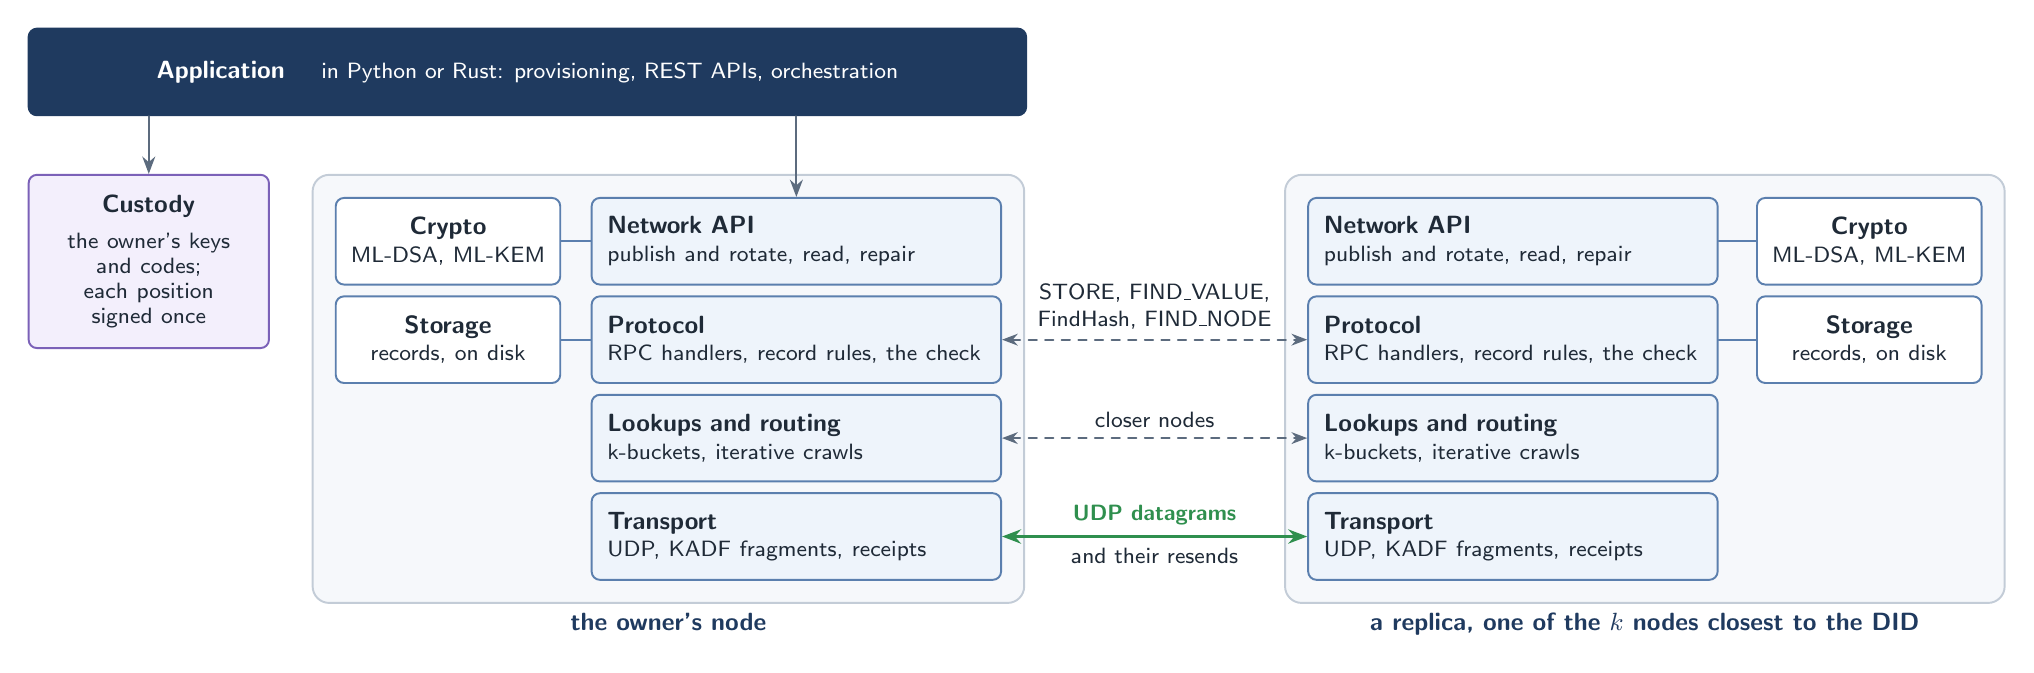
\begin{tikzpicture}[
  layer/.style={public, anchor=north west, minimum width=5.2cm, minimum height=11mm, text width=4.8cm, align=left},
  sidebox/.style={plain, draw=blueLine, anchor=north west, minimum width=2.75cm, minimum height=11mm, text width=2.5cm, align=center},
  peer/.style={dashed, draw=muted, line width=0.7pt, {Stealth[length=2mm]}-{Stealth[length=2mm]}},
  wire/.style={draw=greenLine, line width=1.2pt, {Stealth[length=2.4mm]}-{Stealth[length=2.4mm]}},
  tie/.style={draw=blueLine, line width=0.7pt},
]
  \def\lx{3.9}    % the owner's side column
  \def\ax{7.15}   % the owner's stack
  \def\bx{16.25}  % the replica's stack
  \def\rx{21.95}  % the replica's side column
  \def\top{-2.15} % top of the first layer
  \def\h{1.25}    % row pitch

  % the two stacks
  \foreach \s/\x in {a/\ax, b/\bx} {
    \node[layer] (\s api) at (\x,\top)
      {\textbf{Network API}\\[-1pt] {\footnotesize publish and rotate, read, repair}};
    \node[layer] (\s proto) at (\x,\top-\h)
      {\textbf{Protocol}\\[-1pt] {\footnotesize RPC handlers, record rules, the check}};
    \node[layer] (\s look) at (\x,\top-2*\h)
      {\textbf{Lookups and routing}\\[-1pt] {\footnotesize k-buckets, iterative crawls}};
    \node[layer] (\s trans) at (\x,\top-3*\h)
      {\textbf{Transport}\\[-1pt] {\footnotesize UDP, KADF fragments, receipts}};
  }

  % crypto and storage, on the outer side of each stack
  \foreach \s/\x in {a/\lx, b/\rx} {
    \node[sidebox] (\s crypto) at (\x,\top) {\textbf{Crypto}\\[-1pt] {\footnotesize ML-DSA, ML-KEM}};
    \node[sidebox] (\s store) at (\x,\top-\h) {\textbf{Storage}\\[-1pt] {\footnotesize records, on disk}};
  }
  \draw[tie] (acrypto.east) -- (aapi.west);
  \draw[tie] (astore.east) -- (aproto.west);
  \draw[tie] (bcrypto.west) -- (bapi.east);
  \draw[tie] (bstore.west) -- (bproto.east);

  % the two nodes
  \begin{scope}[on background layer]
    \node[draw=greyLine, fill=greyFill, rounded corners=6pt, line width=0.7pt, inner sep=8pt,
          fit=(acrypto) (atrans)] (anode) {};
    \node[draw=greyLine, fill=greyFill, rounded corners=6pt, line width=0.7pt, inner sep=8pt,
          fit=(bapi) (btrans) (bstore)] (bnode) {};
  \end{scope}
  \node[anchor=north, font=\small\bfseries, text=navy] at (anode.south) {the owner's node};
  \node[anchor=north, font=\small\bfseries, text=navy] at (bnode.south) {a replica, one of the $k$ nodes closest to the DID};

  % the custody beside the owner's node, and the application above both
  \node[secret, anchor=north west, minimum width=3.0cm, minimum height=22mm, text width=2.7cm] (cust)
    at (0,0 |- anode.north)
    {\textbf{Custody}\\[2pt] {\footnotesize the owner's keys}\\[-2pt] {\footnotesize and codes;}\\[-2pt]
     {\footnotesize each position}\\[-2pt] {\footnotesize signed once}};
  \path let \p1 = (anode.east) in
    node[strong, anchor=north west, minimum height=11mm, minimum width=\x1] (app) at (0,0)
    {Application \quad {\normalfont\footnotesize in Python or Rust: provisioning, REST APIs, orchestration}};

  \draw[flow] (app.south -| cust.north) -- (cust.north);
  \draw[flow] (app.south -| aapi.north) -- (aapi.north);

  % what the layers exchange
  \draw[peer] (aproto.east) -- node[data, above=2pt, align=center, fill=none] {STORE, FIND\_VALUE,\\ FindHash, FIND\_NODE} (bproto.west);
  \draw[peer] (alook.east) -- node[data, above=2pt, fill=none] {closer nodes} (blook.west);
  \draw[wire] (atrans.east) -- node[data, above=2pt, text=greenLine, fill=none] {\textbf{UDP datagrams}}
                               node[data, below=2pt, fill=none] {and their resends} (btrans.west);
\end{tikzpicture}
\end{document}
